%!TeX root=../tese.tex
\chapter{Restrições de grau mínimo}
\label{cap:grau-limitado}

% ---------------------------------------
% ------- Vibe coding começa aqui -------
% ---------------------------------------

% Comando personalizado para desenhar o grafo de Andrásfai com parâmetro d
\newcommand{\drawAndrasfai}[1]{%
  \def\d{#1}                              % parâmetro d
  \pgfmathsetmacro\n{int(3*\d - 1)}       % número de vértices n = 3d - 2
  \begin{tikzpicture}[scale=1.5,
    every node/.style={circle, draw, fill=white, inner sep=1pt, font=\small}]
  
  % 1. Coloca os vértices uniformemente em círculo
  \foreach \i in {0,...,\numexpr \n-1 \relax} {
    \pgfmathsetmacro\angle{90-360*\i/\n}
    \node (v\i) at (\angle:1) {\i};       % vértice v_i na posição angular correspondente
  }

  % 2. Para cada vértice, conecta aos d vértices mais distantes
  \foreach \i in {0,...,\numexpr \n-1 \relax} {
    \foreach \offset in {0,...,\numexpr \d-1 \relax} {
      \pgfmathsetmacro\j{mod(\i + \d + \offset, \n)} % vértice mais distante no ciclo
      \pgfmathtruncatemacro{\ii}{\i}
      \pgfmathtruncatemacro{\jj}{\j}
      \ifnum\ii<\jj
        \draw (v\ii) -- (v\jj);          % desenha aresta se ii < jj (para evitar duplicação)
      \fi
    }
  }

  \end{tikzpicture}
}

% --------------------------------------
% ------ Vibe coding termina aqui ------
% --------------------------------------

\newcommand{\homarrow}{\hookrightarrow}

Na literatura de teoria extremal de grafos, o estudo de grafos livres de certas estruturas com grau mínimo limitado inferiormente merece atenção especial.
Um dos teoremas mais fundamentais nesse sentido é o Teorema de Andrásfai-Erd\H os, Sós:
\begin{theorem}[\cite{andrasfai19742n5}]\label{thm:a-e-s}
  Seja $r \geq 2$ e $G$ um grafo livre de $K_{r+1}$ com $n$ vértices.
  Se \[\delta(G) > \frac{3r-4}{3r-1}n,\]
  então $G$ é $r$-partido.
\end{theorem}

Para grafos livres de triângulos, o Teorema~\ref{thm:a-e-s} prova que, se um grafo livre de triângulos tem grau mínimo maior que $\delta(G) > 2n/5$, então ele é bipartido.
Automaticamente, a Conjectura~\ref{conj:make-bipartite} é verdadeira para grafos com grau mínimo maior que $2n/5$.
Mas se $\delta(G) > 2n/5$, então $e(G) > n^2/5$, o que já é coberto pelo Teorema~\ref{thm:n2/5}.
Portanto, é de se perguntar se a condição de grau mínimo pode ser relaxada, a fim de obter algum resultado que não seja automaticamente verdade pela cota em $e(G) \geq n^2/5$.

De fato, essa condição pode ser relaxada:
\begin{theorem}[\cite{brandt2011vega}]~\label{thm:brandt-thomasse}
  Seja $G$ um grafo livre de triângulos com $n$ vértices e $\delta(G) > n/3$.
  Então $\chi(G) \leq 4$.
\end{theorem}
Além disso, o resultado de~\cite{brandt2011vega} permite caracterizar completamente os grafos livres de triângulos e grau mínimo maior que $n/3$ como os grafos homomórficos aos \emph{grafos Vega}.

É interessante observar que a condição do Teorema~\ref{thm:brandt-thomasse} não pode ser substituída por $\delta(G) > cn$ para nenhum $c < 1/3$.
De fato, para todo $\varepsilon > 0$, existem grafos de $n$ vértices com grau mínimo maior que $(1/3-\varepsilon)n$ mas número cromático não limitado (ver~\cite{erdos1973valence}).

O Teorema~\ref{thm:brandt-thomasse} permite descrever exatamente quem são os conjuntos de arestas que podemos remover para calcular $D(G)$ sempre que $\delta(G)>n/3$ usando o Teorema~\ref{thm:simetrizacao}.
Porém, a estrutura dos grafos Vega é não-trivial (o menor deles tem 11 vértices), e por isso iremos restringir a nossa análise a um teorema estrutural mais simples com a restrição adicional de $\chi(G)=3$ ou a restrição de grau mínimo substituída por $\delta(G) > 10n/29$.

Para isso, precisamos definir os grafos de Andrásfai.

\begin{definition}
  Seja $d \geq 1$ um inteiro positivo.
  O \emph{grafo de Andrásfai} $F_d$ é o grafo com vértices $\{0,1,\dots,3d-2\}$ (módulo $3d-1$) e arestas entre $i$ e $i+d+j$ para cada $j \in \{0,1,\dots,d-1\}$.
\end{definition}
Uma forma de representar os grafos de Andrásfai é colocar os vértices em uma circunferência em sentido horário como vértices de $(3d-1)$-ágono regular e ligar cada vértice com os $d$ vértices mais distantes.

\begin{figure}[htbp]
  \centering

  \begin{subfigure}[b]{0.22\textwidth}
    \centering
    \drawAndrasfai{1}
    \caption*{$F_1$}
  \end{subfigure}
  \hfill
  \begin{subfigure}[b]{0.22\textwidth}
    \centering
    \drawAndrasfai{2}
    \caption*{$F_2$}
  \end{subfigure}
  \hfill
  \begin{subfigure}[b]{0.22\textwidth}
    \centering
    \drawAndrasfai{3}
    \caption*{$F_3$}
  \end{subfigure}
  \hfill
  \begin{subfigure}[b]{0.22\textwidth}
    \centering
    \drawAndrasfai{4}
    \caption*{$F_4$}
  \end{subfigure}

  \caption{Grafos de Andrásfai para $d \in \{1,2,3,4\}$. Observe que $F_d$ é $d$-regular e livre de triângulos.}
\end{figure}

No que se segue, para grafos $G$ e $H$, usaremos a notação $G \homarrow H$ para representar que $G$ é homomórfico a $H$ (isto é, $G$ é um subgrafo de um blow-up de $H$).
Os Teoremas~\ref{thm:jin} e~\ref{thm:hom-to-Fd} formam a caracterização estrutural procurada.

\begin{theorem} [\cite{jin199510n29}] \label{thm:jin}
  Seja $G$ um grafo livre de triângulos com $n$ vértices e grau mínimo maior que $10n/29$.
  Então $G \homarrow F_9$.
\end{theorem}

\begin{theorem} [\cite{chen1997triangle}] \label{thm:hom-to-Fd}
  Seja $G$ um grafo livre de triângulos com $n$ vértices e $\chi(G) \leq 3$.
  Se $\delta(G) > \frac{d+1}{3d+2}n$ para algum $d \geq 1$, então $G$ está contido em um blow-up de $F_d$.
\end{theorem}

Do Teorema~\ref{thm:hom-to-Fd}, segue diretamente que se $G$ é um grafo livre de triângulos com $n$ vértices, grau mínimo $\delta(G) > n/3$ e $\chi(G) \leq 3$, então $G$ é homomórfico a algum $F_d$.

\section{A Conjectura~\ref{conj:make-bipartite} para grafos homomórficos a $F_d$}


Em~\cite{mota2019andrasfai}, os autores verificam o seguinte resultado para a Conjectura~\ref{conj:metadinha}:

\begin{theorem}
  Se um grafo $G$ com $n$ vértices é homomórfico a um grafo de Andrásfai $F_d$ para algum $d \geq 1$, então existe $X \subseteq V(G)$ com $|X| \leq \lfloor n/2 \rfloor$ e $e(G[X]) \leq n^2/50$.
\end{theorem}

As técnicas utilizadas em~\cite{mota2019andrasfai} envolvem a representação de grafos de Andrásfai como subgrafos finitos de um grafo infinito com vértices no círculo unitário, e o conjunto $X$ é escolhido de forma geométrica, como a interseção de um intervalo no círculo com os vértices de $G$.

Nessa seção, provamos o seguinte resultado:

\begin{theorem}
  Seja $G$ um grafo livre de triângulos isomorfo a $F_d$ para algum $d \geq 1$.
  Então $G$ satisfaz a Conjectura~\ref{conj:make-bipartite} se alguma das condições abaixo vale:
  \begin{itemize}
    \item $d \leq 4$;
    \item $\alpha(G) = \frac{d}{3d-1}$.
  \end{itemize}
\end{theorem}


A seguir, apresentamos uma prova da Conjectura~\ref{conj:make-bipartite} para grafos homomórficos a $F_4$.
Para começar, apresentamos um lema geral sobre partições do conjunto de arestas em grafos livres de triângulos.

\begin{lemma} \label{lem:odd-transversal}
  Seja $G$ um grafo e suponha que existem conjuntos dois a dois disjuntos $E_1,E_2,E_3,E_4,E_5 \subseteq E$ tais que
  $G-E_i$ é bipartido para cada $i \in \{1,2,3,4,5\}$.
  Então $G$ satisfaz a Conjectura \ref{conj:make-bipartite}.
\end{lemma}

\begin{proof}
  Se $e(G) \geq n^2/5$, então o resultado segue do Teorema \ref{thm:n2/5}.
  Por outro lado, se $e(G) < n^2/5$, então
    \[ 5 \min\{ |E_1|,|E_2|,|E_3|,|E_4|,|E_5| \} \leq |E_1|+|E_2|+|E_3|+|E_4|+|E_5| \leq e(G) < \frac{n^2}{5}, \]
  e para $|E_i| = \min \{ |E_1|,|E_2|,|E_3|,|E_4|,|E_5| \}$ temos $G-E_i$ bipartido com $|E_i| < n^2/5$.
\end{proof}

Dessa forma, se apresentarmos uma tal partição para $F_d$, ela também valerá para qualquer blow-up de $F_d$, independentemente dos tamanhos relativos entre as classes no blow-up.
A figura a seguir mostra que tal partição existe para $F_4$:

  \begin{center}
    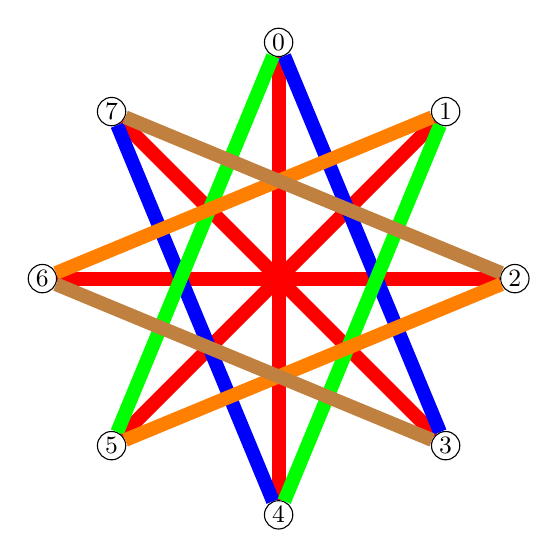
\begin{tikzpicture}[scale=3,
      every node/.style={circle, draw, fill=white, inner sep=1pt, font=\small}]
    
    % 1. Coloca os vértices uniformemente em círculo
    \foreach \i in {0,...,7} {
      \pgfmathsetmacro\angle{90-360*\i/8}
      \node (v\i) at (\angle:1) {\i};       % vértice v_i na posição angular correspondente
    }

    \draw [line width = 5pt, red] (v0)--(v4);
    \draw [line width = 5pt, red] (v1)--(v5);
    \draw [line width = 5pt, red] (v2)--(v6);
    \draw [line width = 5pt, red] (v3)--(v7);

    \draw [line width = 5pt, blue] (v0)--(v3);
    \draw [line width = 5pt, blue] (v7)--(v4);

    \draw [line width = 5pt, green] (v1)--(v4);
    \draw [line width = 5pt, green] (v0)--(v5);

    \draw [line width = 5pt, orange] (v1)--(v6);
    \draw [line width = 5pt, orange] (v2)--(v5);

    \draw [line width = 5pt, brown] (v3)--(v6);
    \draw [line width = 5pt, brown] (v2)--(v7);

    \end{tikzpicture}
  \end{center}



%% Contudo, é fácil ver que tal partição não existe para $F_5$.

O seguinte resultado é imediato da partição acima e dos Teoremas~\ref{thm:jin} e~\ref{thm:hom-to-Fd}.
\begin{corollary}
  Se $G$ é um grafo livre de triângulo com $n$ vértices e $\delta(G) > 4n/11$, então $D(G) \leq \frac{n^2}{25}$.
\end{corollary}

%\begin{proof}
%  Veja que $4/11 > 10/29$, logo pelo Teorema \ref{thm:jin}, temos que $G \homarrow F_9$.
%  Em particular, $\chi(G) \leq \chi(F_9) = 3$.
%  Assim, pelo Teorema \ref{thm:hom-to-Fd} com $d=3$, vale que $G \homarrow F_4$.
%  Considere a seguinte partição das arestas de $G$, em que cada classe está representada por um vértice e todos as arestas entre o mesmo par de classes estão na mesma parte:


%  Como a remoção de cada uma das partes deixa $G$ bipartido, podemos aplicar o Lema \ref{lem:odd-transversal} a $G$.
%  Isso conclui a prova do Teorema. 
%\end{proof}





Vamos tentar resolver quando $\delta(G)$ é grande?
Ok, ok, você vai dizer ``mas o resultado do capítulo 2 já cobre isso''.
Verdade, mas queremos mais \textit{estrutura} sobre os conjuntos que geram $D(G)$, então ainda vale a pena estudar esses casos!